\documentclass{article}

\usepackage{graphicx}
\usepackage{tikz}
\usepackage{tikzsymbols}
\usetikzlibrary{calc,patterns,shapes.geometric}
\pagestyle{empty}
\usepackage[margin=0pt]{geometry}
\geometry{papersize={14in,12in}}

\def\centerarc[#1](#2)(#3:#4:#5){\draw[#1] ($(#2)+({#5*cos(#3)},{#5*sin(#3)})$) arc (#3:#4:#5);}

\begin{document}
	\begin{figure}
		\centering
		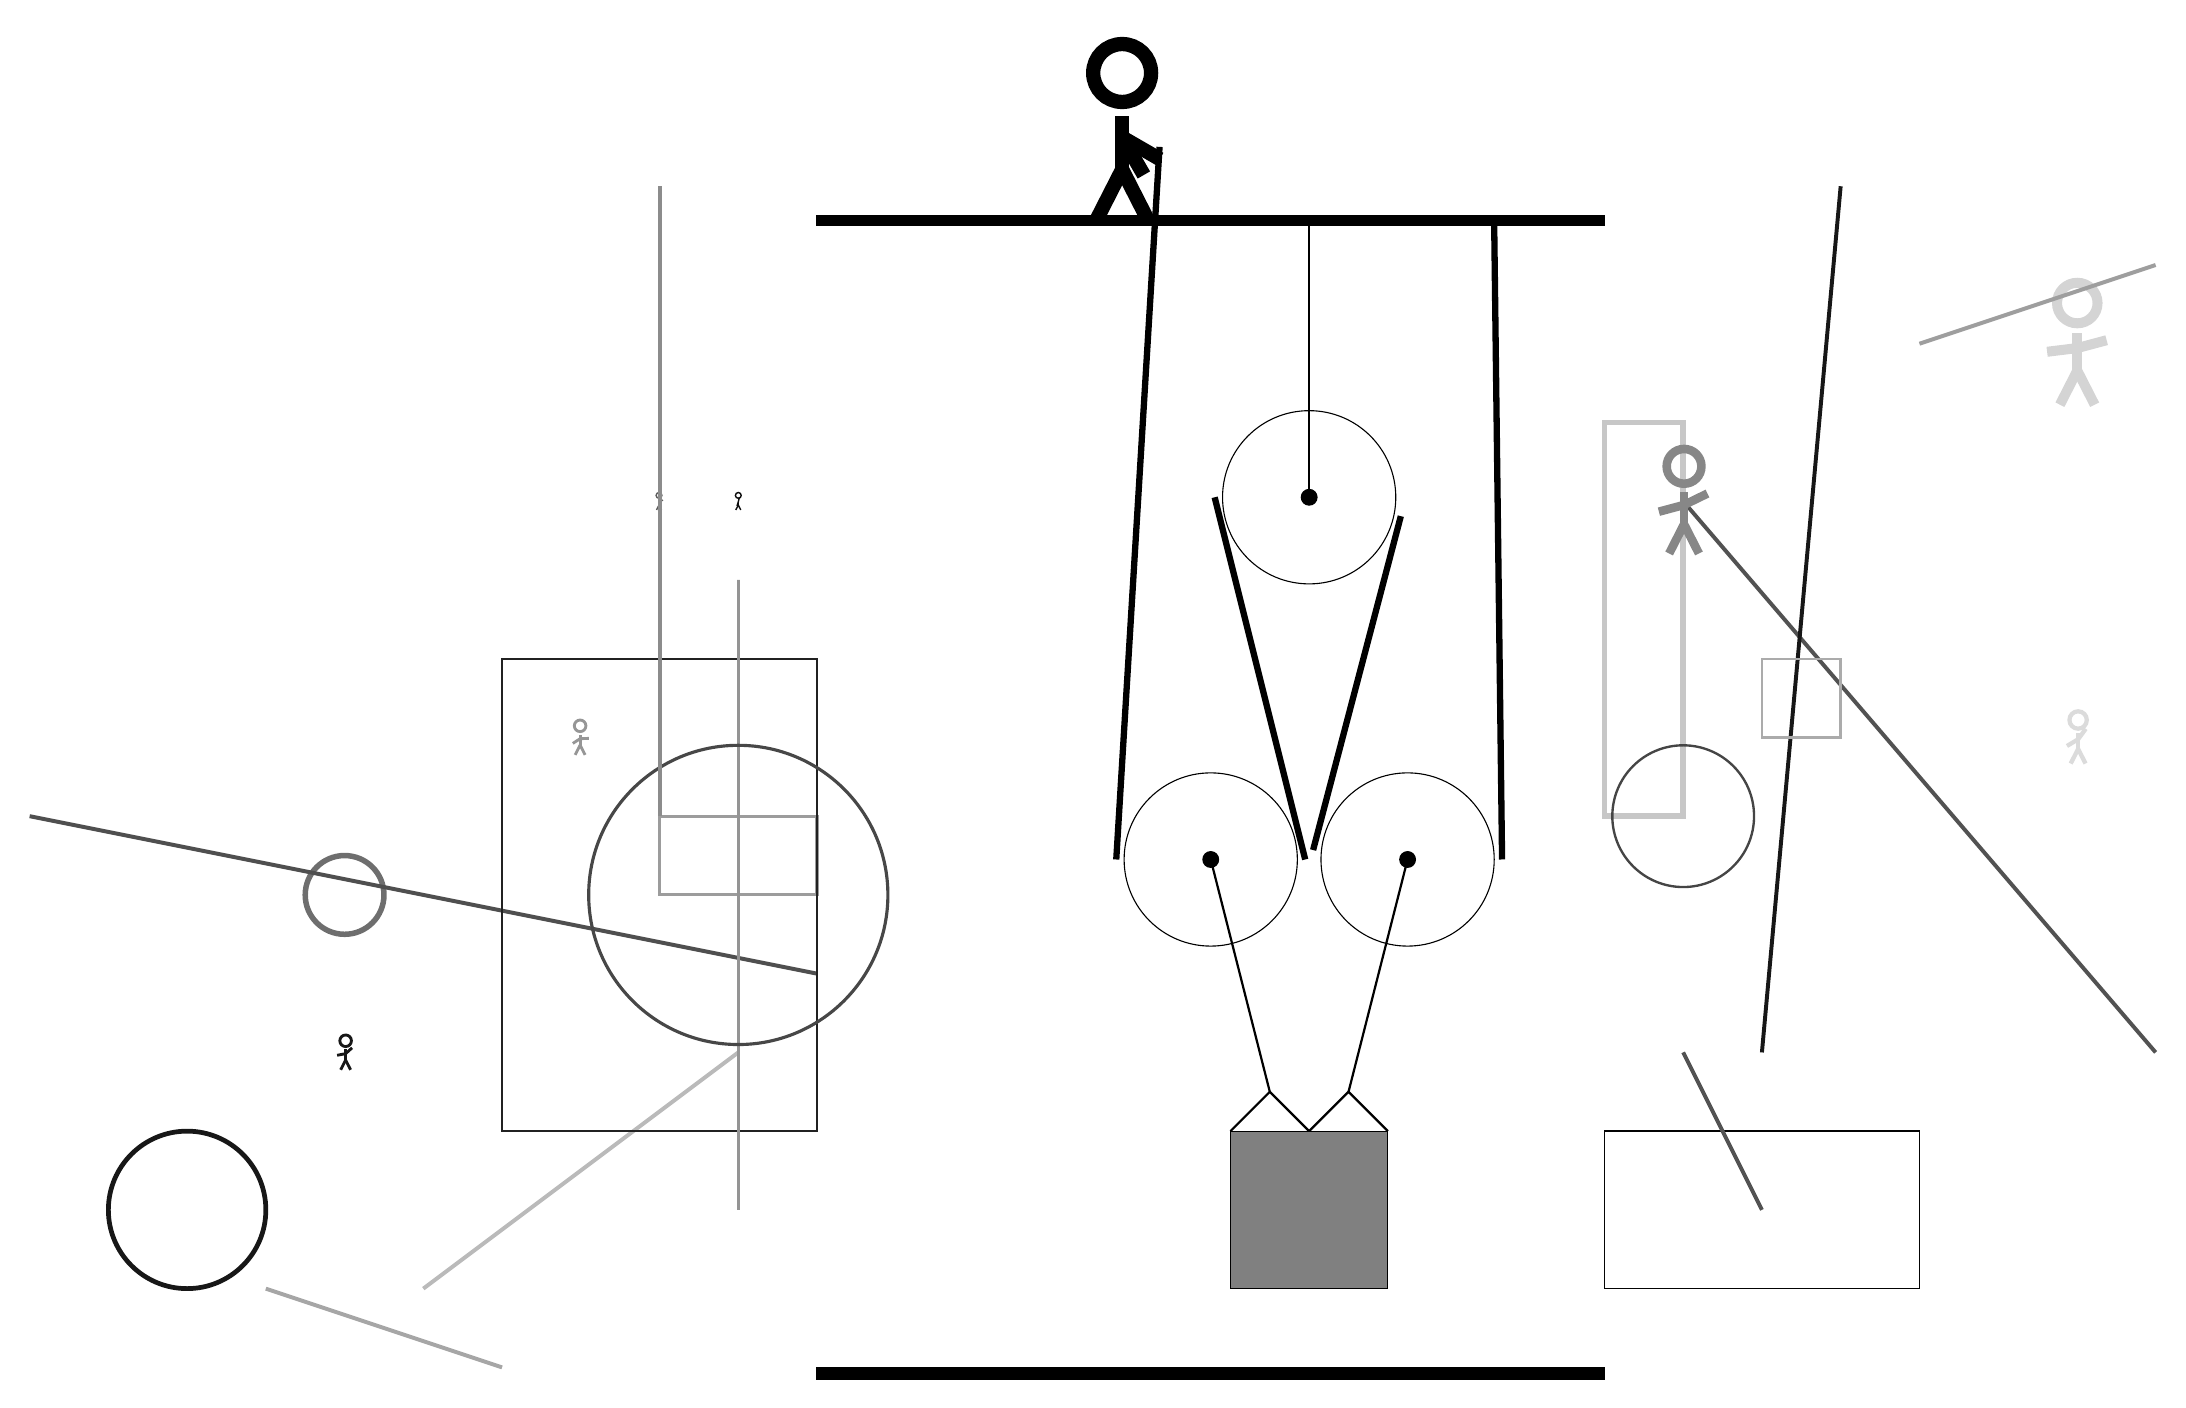
\begin{tikzpicture}
			%%%%% START %%%%%
			
			\draw[fill=black] (-4, 11.5) rectangle (6, 11.625);
			
			\draw (1, 3.45) circle (1.1);
			\draw[fill=black] (1, 3.45) circle (0.1);
			
			\draw [line width=0.7mm, color=black!57](-10, 3) circle (0.5);
			
			\draw[line width=0.5mm, color=black!69](-4, 2) -- (-14, 4);
			\draw[line width=0.2mm, color=black!99] (6, 0) rectangle (10, -2);
			\draw[line width=0.5mm, color=black!35](-8, -3) -- (-11, -2);
			\draw[line width=0.4mm, color=black!39] (-6, 4) rectangle (-4, 3);
			\node[line width=0.6mm, color=black!17] at (12, 10) {\Strichmaxerl[7][7][15]};
			\node[line width=0.6mm, color=black!91] at (-10, 1) {\Strichmaxerl[2][11][42]};
			\node[line width=0.5mm, color=black!14] at (12, 5) {\Strichmaxerl[3][31][54]};
			\draw[line width=0.5mm, color=black!27](-9, -2) -- (-5, 1);
			\draw[line width=0.3mm, color=black!87] (-4, 0) rectangle (-8, 6);
			\draw[line width=0.4mm, color=black!42] (-5, -1) rectangle (-5, 7);
			\draw[line width=0.7mm, color=black!22] (7, 4) rectangle (6, 9);
			\draw [line width=0.6mm, color=black!91](-12, -1) circle (1.0);
			
			\node[line width=0.3mm, color=black!95] at (-5, 8) {\Strichmaxerl[1][73][77]};
			\draw[line width=0.5mm, color=black!68](7, 8) -- (13, 1);
			\node[line width=0.6mm, color=black!47] at (7, 8) {\Strichmaxerl[6][15][26]};
			\node[line width=0.7mm, color=black!64] at (-6, 8) {\Strichmaxerl[1][88][24]};
			\draw [line width=0.3mm, color=black!73](7, 4) circle (0.9);
			\draw [line width=0.4mm, color=black!72](-5, 3) circle (1.9);
			\draw[line width=0.5mm, color=black!91](9, 12) -- (8, 1);
			\draw[line width=0.3mm, color=black!33] (8, 6) rectangle (9, 5);
			\draw[line width=0.5mm, color=black!68](8, -1) -- (7, 1);
			
			\draw[line width=0.5mm, color=black!45](-6, 12) -- (-6, 4);
			\node[line width=0.5mm, color=black!41] at (-7, 5) {\Strichmaxerl[2][33][2]};
			\draw[line width=0.5mm, color=black!38](10, 10) -- (13, 11);
			
			
			\draw (2.25, 8.05) circle (1.1);
			\draw[fill=black] (2.25, 8.05) circle (0.1);
			\draw[thick] (2.25, 8.05) -- (2.25, 11.5);
			
			\draw (3.5, 3.45) circle (1.1);
			\draw[fill=black] (3.5, 3.45) circle (0.1);
			
			\draw[thick] (3.5, 3.45) -- (2.75, 0.5);
			\draw[thick] (1, 3.45) -- (1.75, 0.5);
			\draw[thick]  (1.25, 0) -- (1.75, 0.5) -- (2.25, 0);
			\draw[thick]  (2.25, 0) -- (2.75, 0.5) -- (3.25, 0);
			\draw[fill=black!50] (1.25, 0) rectangle (3.25, -2);
			
			\draw[line width=0.8mm] (0.35, 12.5) --  (-0.2, 3.45);
			\centerarc[line width=0.8mm](1, 3.45)(180:360:1.2000000000000002);
			\draw[line width=0.8mm] (2.2, 3.45) -- (1.05, 8.05);
			\centerarc[line width=0.8mm](2.25, 8.05)(-20:180:1.2000000000000002);
			\draw[line width=0.8mm](3.414, 7.81) -- (2.3, 3.57);
			\centerarc[line width=0.8mm](3.5, 3.45)(160:360:1.2000000000000002);
			\draw[line width=0.8mm](4.7, 3.45) -- (4.6, 11.5);
			
			\node at (-0.07, 12.7) {\Strichmaxerl[10][120][-30]};
			
			\draw[fill=black] (-4, -3) rectangle (6, -3.15);
			
			%%%%% END %%%%%
		\end{tikzpicture}
	\end{figure}	
\end{document}